\documentclass [tikz] {standalone}

\input{header.htex}

\begin {document}


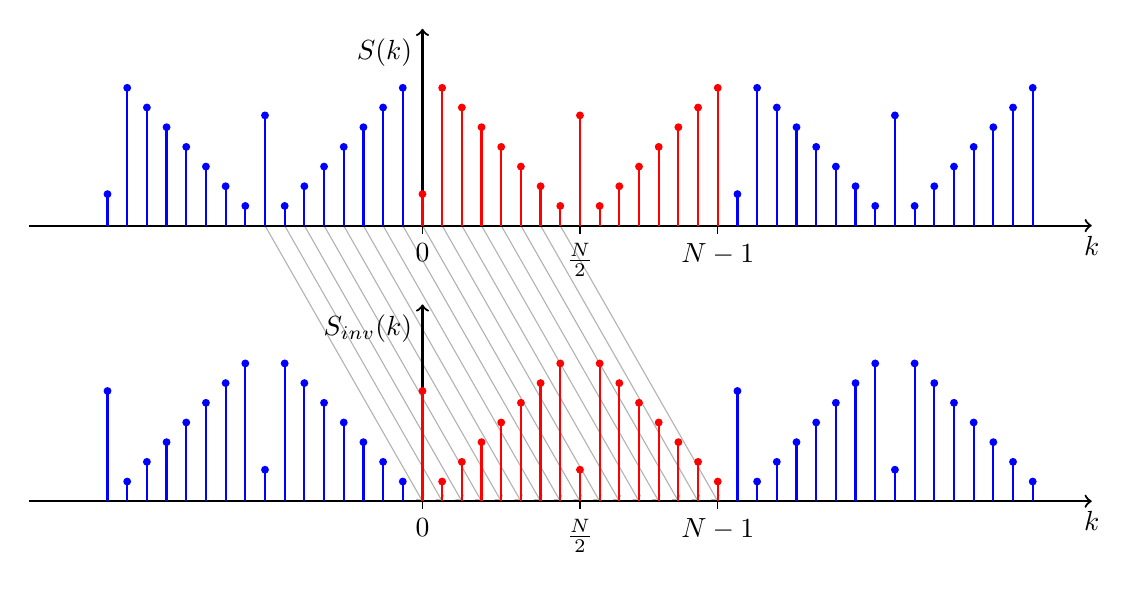
\begin{tikzpicture}

%\draw [->, thin, draw = white!70!black] (0 , 0cm) -- (2 , -3.5);
%\draw [->, thin, draw = white!70!black] (2 , 0cm) -- (0 , -3.5);

\foreach \z in { 0, 1, ..., 15}
{	
	\draw [->, thin, draw = white!70!black] (\z * 0.25 - 2 , 0cm) -- (\z * 0.25 , -3.5);
	
	
	
}



\draw[->,thick] (-5cm,	0cm)		-- (8.5cm, 0cm)	node[below] {$k$};
\draw[->,thick] ( 0cm,	0cm)		-- (   0cm, 2.5cm)	node[below left] {$S(k)$};
\draw[-, thin] (0, 0) -- (0, -0.1) node[below] {$0$};
\draw[-, thin] (2, 0) -- (2, -0.1) node[below] {$\frac{N}{2}$};
\draw[-, thin] (3.75, 0) -- (3.75, -0.1) node[below] {$N-1$};


\draw[->,thick] (-5cm,	-3.5cm)		-- (8.5cm, -3.5cm)	node[below] {$k$};
\draw[->,thick] ( 0cm,	-3.5cm)		-- (   0cm, -1cm)	node[below left] {$S_{\text{inv}}(k)$};
\draw[-, thin] (0, -3.5) -- (0, -3.6) node[below] {$0$};
\draw[-, thin] (2, -3.5) -- (2, -3.6) node[below] {$\frac{N}{2}$};
\draw[-, thin] (3.75, -3.5) -- (3.75, -3.6) node[below] {$N-1$};


\draw[-, thick, draw = red] (0, 0) -- (0, 0.4);
\fill[fill = red] (0, 0.4 ) circle(0.05cm);
\draw[-, thick, draw = red] (2, 0) -- (2, 1.4);
\fill[fill = red] (2, 1.4 ) circle(0.05cm);

\draw[-, thick, draw = blue] (-4, 0) -- (-4, 0.4);
\fill[fill = blue] (-4, 0.4 ) circle(0.05cm);
\draw[-, thick, draw = blue] (-2, 0) -- (-2, 1.4);
\fill[fill = blue] (-2, 1.4 ) circle(0.05cm);


\draw[-, thick, draw = blue] (4, 0) -- (4, 0.4);
\fill[fill = blue] (4, 0.4 ) circle(0.05cm);
\draw[-, thick, draw = blue] (6, 0) -- (6, 1.4);
\fill[fill = blue] (6, 1.4 ) circle(0.05cm);


\draw[-, thick, draw = red] (0, -3.5) -- (0, -2.1);
\fill[fill = red] (0, -2.1 ) circle(0.05cm);
\draw[-, thick, draw = red] (2, -3.5) -- (2, -3.1);
\fill[fill = red] (2, -3.1 ) circle(0.05cm);

\draw[-, thick, draw = blue] (-4, -3.5) -- (-4, -2.1);
\fill[fill = blue] (-4, -2.1 ) circle(0.05cm);
\draw[-, thick, draw = blue] (-2, -3.5) -- (-2, -3.1);
\fill[fill = blue] (-2, -3.1 ) circle(0.05cm);

\draw[-, thick, draw = blue] (4, -3.5) -- (4, -2.1);
\fill[fill = blue] (4, -2.1 ) circle(0.05cm);
\draw[-, thick, draw = blue] (6, -3.5) -- (6, -3.1);
\fill[fill = blue] (6, -3.1 ) circle(0.05cm);


\foreach \z in { 1, 2, ..., 7}
{	
	\draw [thick, draw = red] (\z * 0.25 , 0cm) -- (\z * 0.25 , 2.0 - \z*0.25);	\fill[fill = red] (\z * 0.25 , 2.0 - \z*0.25 ) circle(0.05cm);
		
	
	\draw [thick, draw = red] (\z * 0.25 + 2 , 0cm) -- (\z * 0.25 + 2 , \z*0.25);
	\fill[fill = red] (\z * 0.25 + 2 , \z*0.25 ) circle(0.05cm);
	
	\draw [thick, draw = blue] (\z * 0.25 - 2 , 0cm) -- (\z * 0.25 - 2 , \z*0.25);
	\fill[fill = blue] (\z * 0.25- 2 , \z*0.25 ) circle(0.05cm);
	\draw [thick, draw = blue] (\z * 0.25 +6 , 0cm) -- (\z * 0.25 +6 , \z*0.25);
	\fill[fill = blue] (\z * 0.25+6 , \z*0.25 ) circle(0.05cm);
	
	
	\draw [thick, draw = blue] (\z * 0.25+4 , 0cm) -- (\z * 0.25+4 , 2.0 - \z*0.25);	\fill[fill = blue] (\z * 0.25 +4, 2.0 - \z*0.25 ) circle(0.05cm);
	
	\draw [thick, draw = blue] (\z * 0.25-4 , 0cm) -- (\z * 0.25-4 , 2.0 - \z*0.25);	\fill[fill = blue] (\z * 0.25-4 , 2.0 - \z*0.25 ) circle(0.05cm);
	
	
	
	\draw [thick, draw = red] (\z * 0.25 , -3.5cm) -- (\z * 0.25 , \z*0.25 - 3.5);
	\fill[fill = red] (\z * 0.25 , \z*0.25 - 3.5 ) circle(0.05cm);
	
	\draw [thick, draw = blue] (\z * 0.25-2  , -3.5cm) -- (\z * 0.25-2 , 2.0 - \z*0.25 -3.5);
	\fill[fill = blue] (\z * 0.25-2 , 2.0 - \z*0.25 -3.5 ) circle(0.05cm);
	
	\draw [thick, draw = blue] (\z * 0.25+6  , -3.5cm) -- (\z * 0.25+6, 2.0 - \z*0.25 -3.5);
	\fill[fill = blue] (\z * 0.25+6 , 2.0 - \z*0.25 -3.5 ) circle(0.05cm);
			
		
	\draw [thick, draw = red] (\z * 0.25 + 2 , -3.5cm) -- (\z * 0.25 +2 , -1.5 - \z*0.25);
	\fill[fill = red] (\z * 0.25 +2 , -1.5 - \z*0.25) circle(0.05cm);
	
	
	\draw [thick, draw = blue] (\z * 0.25 + 4 , -3.5cm) -- (\z * 0.25 + 4 , \z*0.25-3.5);
	\fill[fill = blue] (\z * 0.25 + 4 , \z*0.25 -3.5) circle(0.05cm);
		
	\draw [thick, draw = blue] (\z * 0.25 - 4 , -3.5cm) -- (\z * 0.25 - 4 , \z*0.25-3.5);
	\fill[fill = blue] (\z * 0.25 - 4 , \z*0.25 -3.5) circle(0.05cm);

	
}



\end{tikzpicture}
\end {document}
%		\caption{Инверсия спектра сигнала за счет частотного сдвига}\label{dftprop:fig3}
%	\end{center}
%\end{figure}
